\section{Ferramentas e Plataformas usadas no desenvolvimento da RIL}

    Nesta secção vão ser analisadas as ferramentas usadas no projeto, e que equipas ou profissionais é que normalmente as manuseiam e como.

    \subsection{OutSystems}\label{sec:outsystems}
    
        Estabelecida em 2001, a OutSystems é uma das principais plataformas mencionadas no desenvolvimento \textit{low-code}, foi desenhada com um fluxo empresarial em mente, facilitando a criação e entrega rápida de aplicações. A sua interface de desenvolvimento visual permite a construção de aplicações usando modelos visuais, ações, módulos e blocos reutilizáveis, e diferencia-se oferecendo um conjunto abrangente de ferramentas que cobrem todo o ciclo de vida da aplicação\cite{os-vision}.

        \begin{comment}
            !! Fazer um artigo sobre criar uma aplicação low code com recurso a mongoDB e azure.
            Artigo, o ISEC ajuda a pagar.
        
            Fazer aplicação para o relatorio. 
        
            a gente usa o Azure Devops para ver os repos
        
            (Tem que have sempre texto aqui)
        \end{comment}
                    
        %\subsubsection{Service Studio}

    O Service Studio é o ambiente de desenvolvimento low-code de OutSystems, é onde se criam as aplicações, módulos e a lógica por detrás destas, bem como o desenvolvimento das interfaces de utilizadores para aplicações, quer sejam web tradicionais, web reativas ou móveis. 
    É neste ambiente também que se definem os modelos das bases de dados internas a OS. 
    
    É uma ferramenta muito importante no contexto dário para o desenvolvimento e manutenção cotínua da aplicação.

\subsubsection{Service Center}

    A plataforma oferece uma variedade de configurações que podem ser ajustadas para personalizar o comportamento em diferentes áreas. Estas configurações são ajustáveis a partir do Service Center, permitindo a visualização e gestão de uma panóplia de funcionalidades como módulos e dependências entre eles, gestão das diferentes aplicações do projeto, gestão do versionamento de cada módulo através da publicação da versão desejada. Bem como o ajuste de variáveis globais.
    
    O Service Center é também uma ferramenta essencial para gerir e diagnosticar erros durante o desenvolvimento ou manutenção, permitindo visualizar logs relacionados com timers, processos, módulos, \textit{screen requests}, \textit{service actions}, \textit{traditional web requests}, integrações, extensões ou e-mails.

\subsubsection{Lifetime}

    O Lifetime é uma plataforma do ecossistema de OutSystems que gere o ciclo de vida completo das aplicações. Proporciona visibilidade total sobre os diferentes ambientes, desde o desenvolvimento até à produção, sendo a ferramenta principal na realização de \textit{Deployments}, resolvendo conflitos e efetuando \textit{merges} automaticamente sempre que possível e ajudando o utilizador no processo em caso de conflitos. Oferece, além disso, funcionalidades para versionamento e migração.

        \subsubsection{Um Guia de Boas Práticas de Código para OutSystems}\label{secsec:um-guia-de-estilo-de-codigo}

    Todas as linguagens de programação bem estabelecidas têm diretrizes de programação tão bem enraizadas na cultura da língua que são ensinadas em conjunto com ela, desta forma, com os profissionais a aplicar um método parecido no desenvolvimento do código tem-se um projeto muito mais coerente.

    No entanto, OutSystems carece de um guia de diretrizes estabelecido. Isto deve-se principalmente ao facto de OutSystems ser radicalmente diferente de outras linguagens de programação, sendo um paradigma visual onde até a interface pode ser modificada, não existe um consenso universal para a forma como o código deva ser organizado visualmente.

    Neste capítulo vamos explorar algumas das diretrizes que nos foram introduzidas e aconselhadas a seguir quando alterássemos código na aplicação. Estas indicações começaram a ser introduzidas recentemente, pelo que muito do código existente não cumpre estas normas, mas há um incentivo para uniformizar o código da aplicação.

    \textbf{Diretriz 1 — Sentido descendente é progresso:} Figura \ref{fig:diretriz1}, o sentido descendente deve levar-nos ao objetivo da ação. Este é o sentido de leitura geralmente acordada, até por diferentes culturas;

    \textbf{Diretriz 2 — Ramificações para a direita:} Figura \ref{fig:diretriz2}, o ramo mais importante de um ``if'' deverá seguir da esquerda para a direita. Um nodo ``if'' geralmente tem um ramo que se espera ser executado com mais frequência ou o ramo que é simplesmente mais importante a termos de valor comercial. Este ramo deve mover-se para a direita, e o outro deve continuar reto para baixo;

    \begin{figure}[H]
        \centering
        \begin{minipage}{.5\textwidth}
            \centering
            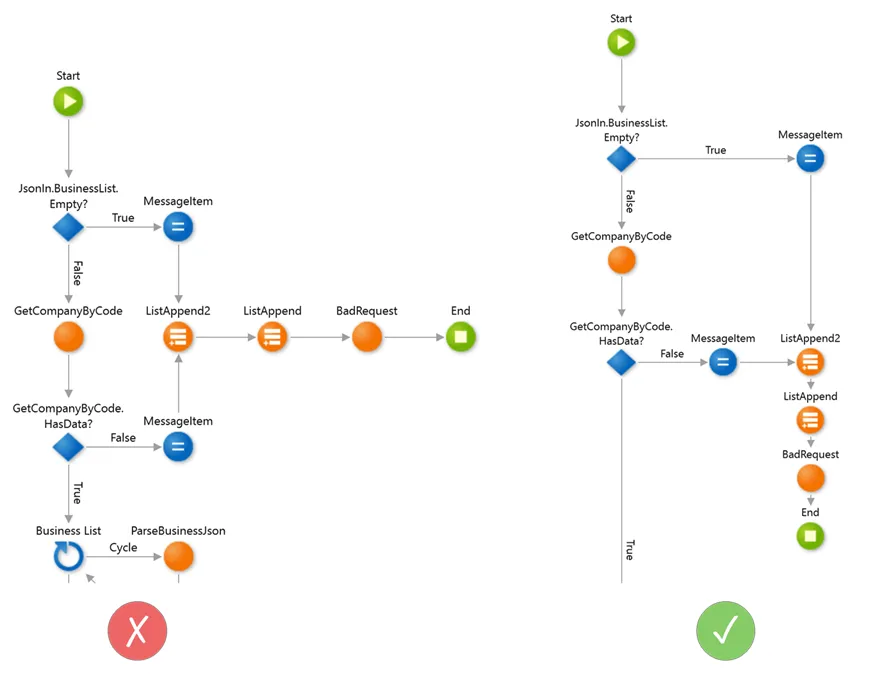
\includegraphics[scale=0.35]{imgs/diretrizes/1.png}
            \caption{Diretriz 1 — Sentido descendente é progresso}\label{fig:diretriz1}
            \source{\cite{outsystems-style-guide}}
        \end{minipage}%
        \begin{minipage}{.5\textwidth}
            \centering
            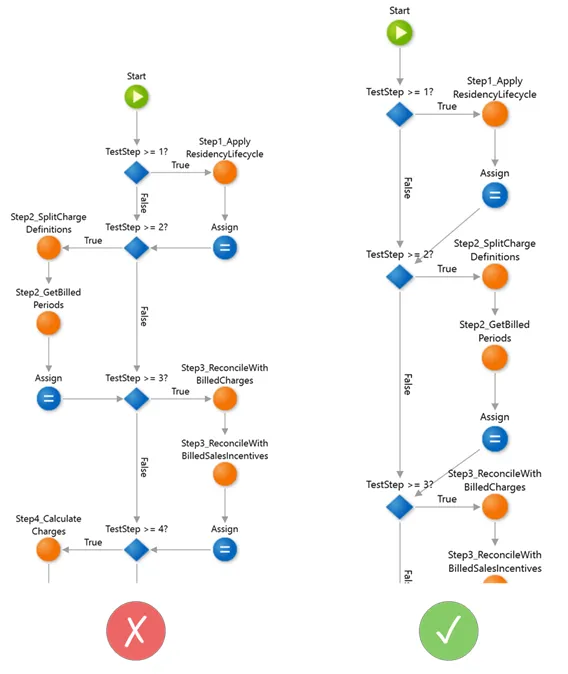
\includegraphics[scale=0.40]{imgs/diretrizes/2.png}
            \caption{Diretriz 2 — Ramificações para a direita}\label{fig:diretriz2}
            \source{\cite{outsystems-style-guide}}
        \end{minipage}
    \end{figure}

    \textbf{Diretriz 3 — Exceções para a direita:} Figura \ref{fig:diretriz3}, exceções para a direita, mesmo que não seja o ramo ``mais importante''. Se se aplicasse a diretriz 2 às exceções, acabava-se com um código maioritariamente horizontal, desta forma impede-se que a exceção se destaque, e mantém-se o foco no código principal;

    \textbf{Diretriz 4 — Ciclos:} Figura \ref{fig:diretriz4}, os ciclos devem iniciar-se numa diagonal para cima e para a direita;

    \begin{figure}[htbp]
        \centering
        \begin{minipage}{.5\textwidth}
            \centering
            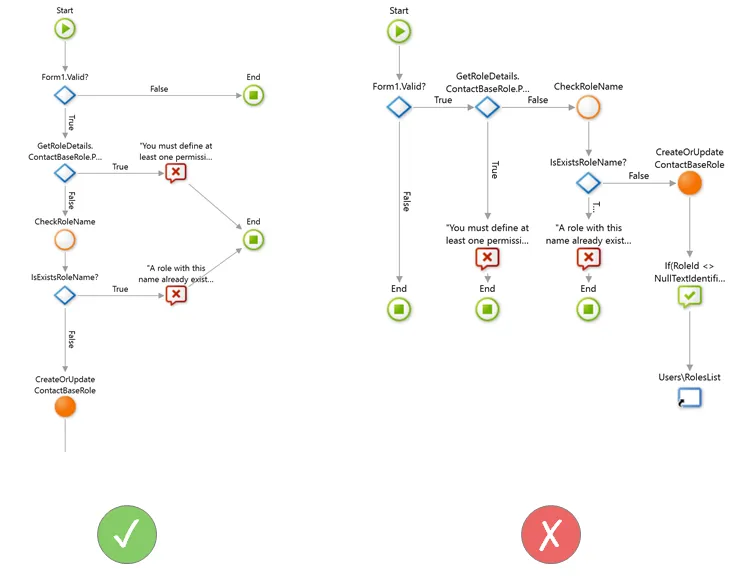
\includegraphics[scale=0.40]{imgs/diretrizes/3.png}
            \caption{Diretriz 3 — Exceções para a direita}\label{fig:diretriz3}
            \source{\cite{outsystems-style-guide}}
        \end{minipage}%
        \begin{minipage}{.5\textwidth}
            \centering
            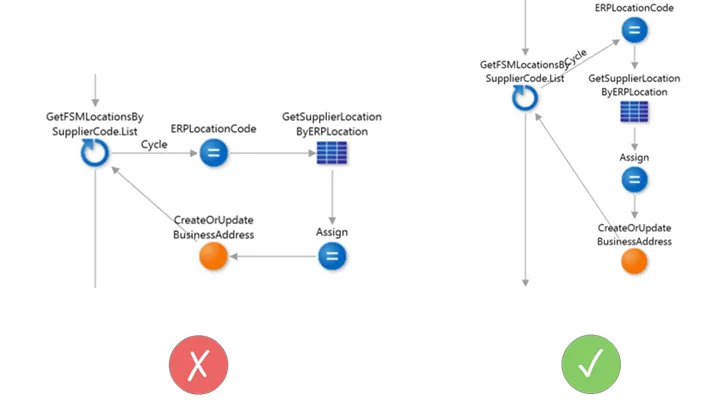
\includegraphics[scale=0.32]{imgs/diretrizes/4.png}
            \caption{Diretriz 4 — Ciclos}\label{fig:diretriz4}
            \source{\cite{outsystems-style-guide}}
        \end{minipage}
    \end{figure}

    \textbf{Diretriz 5 — Evitar setas sobrepostas:} Figura \ref{fig:diretriz5}, as setas sobrepostas devem ser evitadas mesmo que implique ignorar outra diretriz, se for necessário deve-se criar nodos ``dummy'' para direcionar as setas de forma a que não se sobreponham;

    \textbf{Diretriz 6 — Alinhar com intenção:} Figura \ref{fig:diretriz6}, alinhar intencionalmente os nodos relacionados entre si. Por exemplo, se dois ramos têm código similar, os nodos iguais devem estar alinhados horizontalmente para ser ver que será o mesmo código;

    \begin{figure}[htbp]
        \centering
        \begin{minipage}{.5\textwidth}
            \centering
            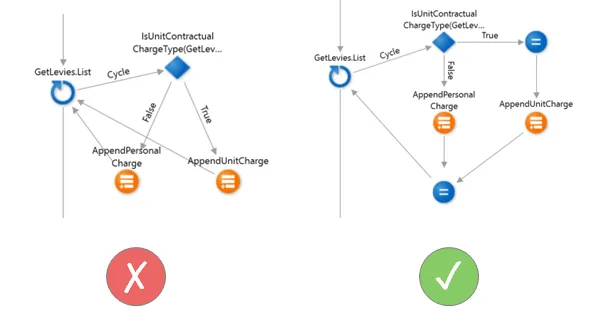
\includegraphics[scale=0.37]{imgs/diretrizes/5.png}
            \caption{Diretriz 5 — Evitar sobreposições}\label{fig:diretriz5}
            \source{\cite{outsystems-style-guide}}
        \end{minipage}%
        \begin{minipage}{.5\textwidth}
            \centering
            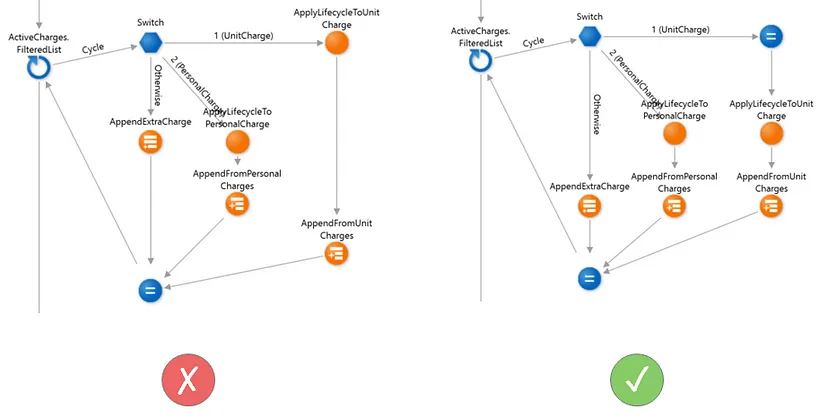
\includegraphics[scale=0.30]{imgs/diretrizes/6.png}
            \caption{Diretriz 6 — Alinhar com intenção}\label{fig:diretriz6}
            \source{\cite{outsystems-style-guide}}
        \end{minipage}
    \end{figure}

    Com estas 6 diretrizes é mais fácil organizar e ler o código da plataforma, e permitirá ter um projeto mais homogéneo e previsível\cite{outsystems-style-guide}.

    % Outlook e ferramentas de desenvolvimento


    % todo, in the Infrestrutura tecnologica na secção que fala de Atlas, referencia também esta secção

        \subsubsection{Competidores}\label{secsec:competidores}

    No ecossistema de desenvolvimento \textit{low-code}, existem várias plataformas que competem com OutSystems. A escolha entre estas dependerá das necessidades específicas de cada projeto, das preferências da equipa e das metas da empresa. 

    Apesar de OutSystems ser uma das plataformas mais maduras e bem desenvolvidas para este fim no mercado, podemos fazer uma análise dos seus pontos fortes e fracos:

    \textbf{Pontos Fortes:}
    \begin{itemize}
        \item O Controlo de versionamento pode ser integrado com Git e plataformas como GitHub ou GitLab;
        \item Várias opções para integração com outras plataformas com ferramentas como o \href{https://integrationbuilder.outsystems.com/}{Integration Builder}, desde servidores SQL ao MS SharePoint Online;
        \item Vastas livrarias, pré-definições, e templates disponíveis;
        \item Ênfase também no desenvolvimento de aplicações móveis.
    \end{itemize}

    \textbf{Pontos Fracos:}
    \begin{itemize}
        \item Uma personalização de UI menos flexível em comparação com algumas alternativas;
        \item Flexibilidade para correr os próprios servidores está apenas disponível em alguns planos;
        \item Colaboração não é um dos aspetos mais fortes da plataforma;
        \item Custo comparativamente elevados em relação a outras alternativas\cite{outsystems-vs-mendix}.
    \end{itemize}

    Na Figura \ref{fig:googletrendslowcodeplatforms-ui} pode-se ver algumas das plataformas \textit{low-code} mais usadas nos últimos cinco anos de acordo com o Google Trends e na Figura \ref{tab:lowcode-comparison} como se comparam com as demais.

    \begin{figure}[p] % htbp
        \centering
        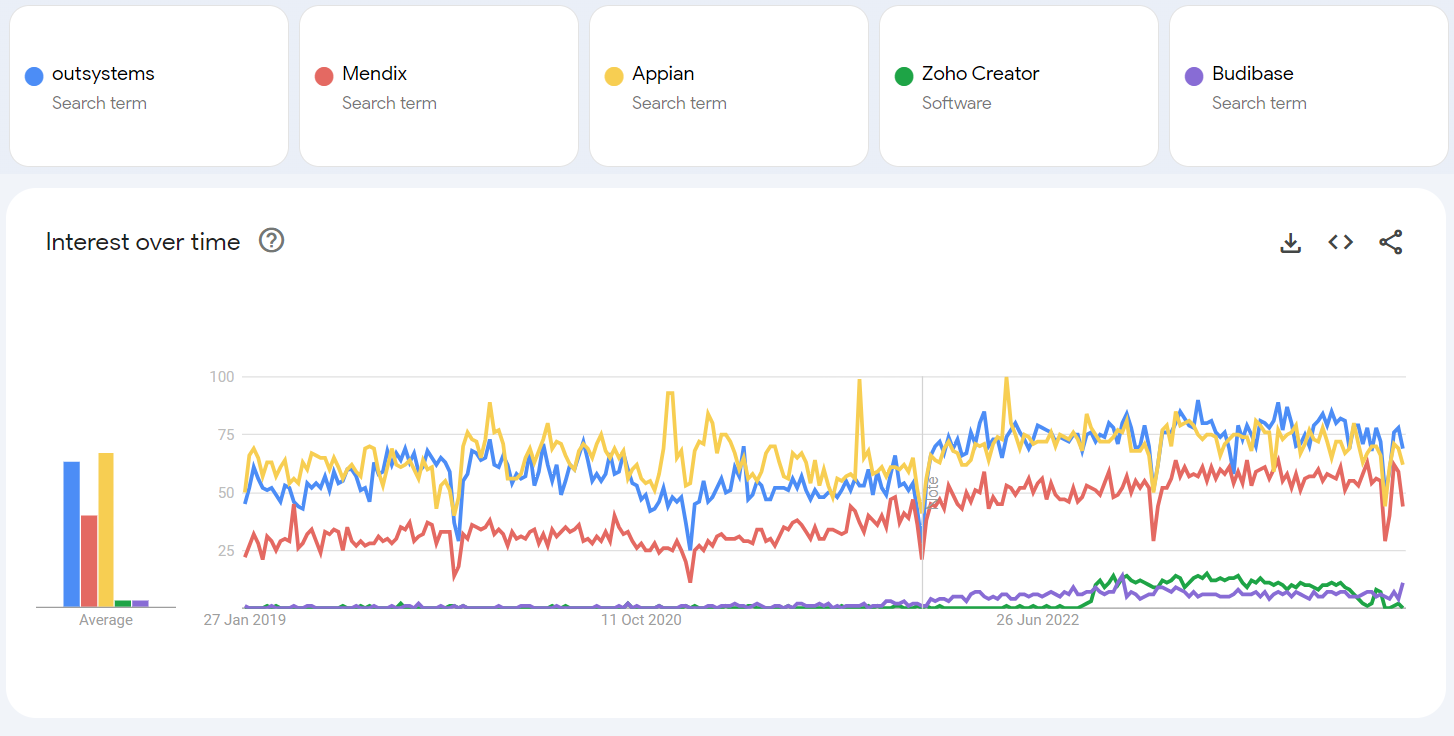
\includegraphics[width=\textwidth]{imgs/GoogleTrendsLowCodePlatforms.png}
        \caption{Google Trends for Low Code Platforms Worldwide}\label{fig:googletrendslowcodeplatforms-ui}
        \source{\cite{g-trends-low-code-platforms}}
    \end{figure}

    % Use this to finish the table: https://impalaintech.com/blog/mendix-vs-outsystems-vs-appian/

    \begin{table}[p] % htbp
        \centering
        \begin{tblr}{
            % example for tblr: https://tex.stackexchange.com/questions/603349/tabularray-and-new-command-for-multicolumn-cells
            % another example: https://tex.stackexchange.com/questions/605676/tabularray-how-to-control-the-vertical-alignment-of-the-cells-contents
            hlines={lightgray}, vlines={lightgray},
            width = \linewidth,% total width set to width available
            %rows = {c,m}, % c aligns horizontally, m aligns vertically, aligns all rows
            colspec={Q[l,m,3cm] X[c,m] X[c,m] X[c,m] X[c,m]},
            cell{1}{1} = {r=2}{c}, % Merge cells in the first row and second row
        }
            \textbf{Campo} & \SetCell[c=4]{c} \textbf{Plataformas} \\
                        & \textbf{OutSystems} & \textbf{Mendix} & \textbf{Appian} & \textbf{Pega} \\ 
            Facilidade de Utilização               & Médio       & Alto        & Alto        & Baixo        \\ 
            Integração                             & Muito Alto  & Alto        & Alto        & Alto        \\ 
            Escalabilidade                         & Muito Alto  & Muito Alto  & Muito Alto  & Muito Alto  \\ 
            % Flexibilidade no Desenvolvimento da UI & Alto        & Muito Alto  & Alto        & Alto        \\  % Para Pega e Appian são as unicas duas que não estão bem fundamentadas
            Foco em Desenvolvimento Móvel          & Alto        & Alto        & Alto        & Alto        \\ 
            Colaboração                            & Alto        & Muito Alto  & Alto        & Alto       \\
            Custo                                  & Alto        & Disponível após Pedido & Alto & Disponível após Pedido  \\
        \end{tblr}
        \caption{Comparação de Plataformas Low-Code}
        \label{tab:lowcode-comparison}
        \source{\cite{mendix-vs-outsystems-vs-appian,outsystems-vs-mendix}} % 1- https://impalaintech.com/blog/mendix-vs-outsystems-vs-appian/
    \end{table}

    O ambiente de desenvolvimento \textit{low-code} é muito competitivo, pelo que existe uma panóplia de ferramentas com objetivos similares, como por exemplo: Bonitasoft, Appsheet, Bubble, Zoho Create, Budibase, Backendless, Eclipse/SAP, Salesforce Lightning, etc. Pode ser que nenhuma das ferramentas aqui analisadas sejam a mais indicada para qualquer projeto. Algumas equipas também adotam abordagens com uma pilha de infraestrutura constituída por vários programas de ecossistemas diferentes, utilizando diferentes ferramentas para aspetos específicos, como Webflow para o front-end e Zappier ou N8n para o lado do servidor. No fundo, esta área é muito flexível e está sempre em constante evolução, e pode ser que a infraestrutura mais indicada para um projeto seja uma que tenha que ser feita à medida.
        
    % Reddit opinion: https://www.reddit.com/r/lowcode/comments/lp9f4p/recommendations_please/
    % Outras: Bonitasoft, Appsheet, bubble, Zoho Create, Budibase, Backendless and Eclipse/SAP, Salesforce Lightning
    % ou uso de várias: Webflow is relatively powerful for a front-end, Zappier or N8n (free) - for the server side, and some database (tool) - Airtable/Firebase/Backendless - for the data.
    % outra dessas arranjei aqui: https://www.outsystems.com/forums/discussion/86088/outsystems-vs-other-low-code-platforms/

    % Another reddit opinion: https://www.reddit.com/r/lowcode/comments/lp9f4p/recommendations_please/


    \subsubsubsection{Mendix}\label{secsecsec:mendix}
        
        Fundada em 2005, a Mendix é uma plataforma de desenvolvimento \textit{low-code} projetada para fornecer às empresas ferramentas para rapidamente construir e distribuir aplicações personalizadas. Os fundadores acreditavam que o desenvolvimento e a distribuição de software iria beneficiar bastante com uma mudança de paradigma, e daí nasceu a empresa. Mendix foca-se na colaboração permitindo às equipas trabalhar efetivamente em conjunto e simplificando o desenvolvimento através de modelagem visual com uma interface intuitiva, como visivel na Figura \ref{fig:mendixui-ui}, e componentes reutilizáveis\cite{why-was-mendix-founded}.

        O Mendix destaca-se pela sua flexibilidade enquanto mantém um bom nível de intuição. Oferece também um mercado privado de aplicações que permite a sua partilha mesmo internamente. Proporciona uma variedade de opções de implementação, incluindo diferentes serviços cloud, soluções locais e híbridas, adaptando-se sempre às diversas necessidades da organização\cite{outsystems-vs-mendix}.

        \begin{figure}[htbp] % htbp
            \centering
            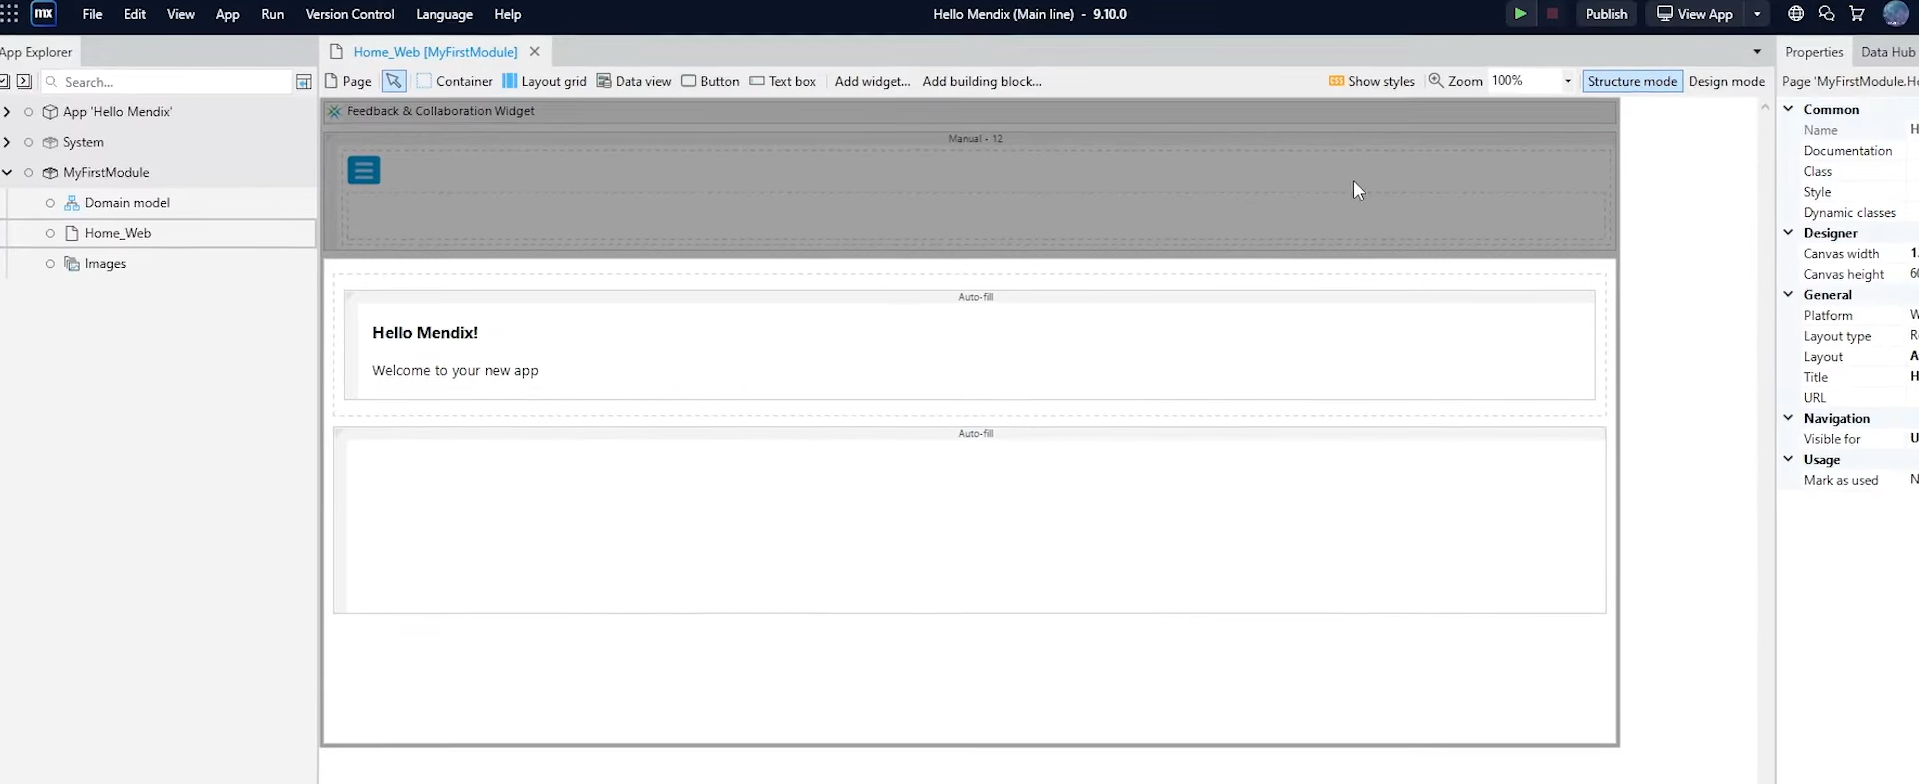
\includegraphics[width=\textwidth]{imgs/MendixUI.png}
            \caption{Mendix UI}\label{fig:mendixui-ui}
            \source{\cite{mendix-ui}}
        \end{figure}

        % https://www.appsmith.com/blog/mendix-vs-outsystems

    \subsubsubsection{Appian}\label{secsec:appian}

        Fundada em 1999 por Michael Beckley, Robert Kramer, Marc Wilson e Matthew Calkins e com uma interface como observável na Figura \ref{fig:appian-ui}, a Appian é uma plataforma de desenvolvimento \textit{low-code} criada com o objetivo de simplificar e acelerar o processo de desenvolvimento de software e com a visão de que pessoas talentosas e com paixão, quando proporcionadas com as ferramentas certas irão dar resultados incríeis\cite{appian-company-history,appian-company-overview}. 
    
        \begin{figure}[htbp] % htbp
            \centering
            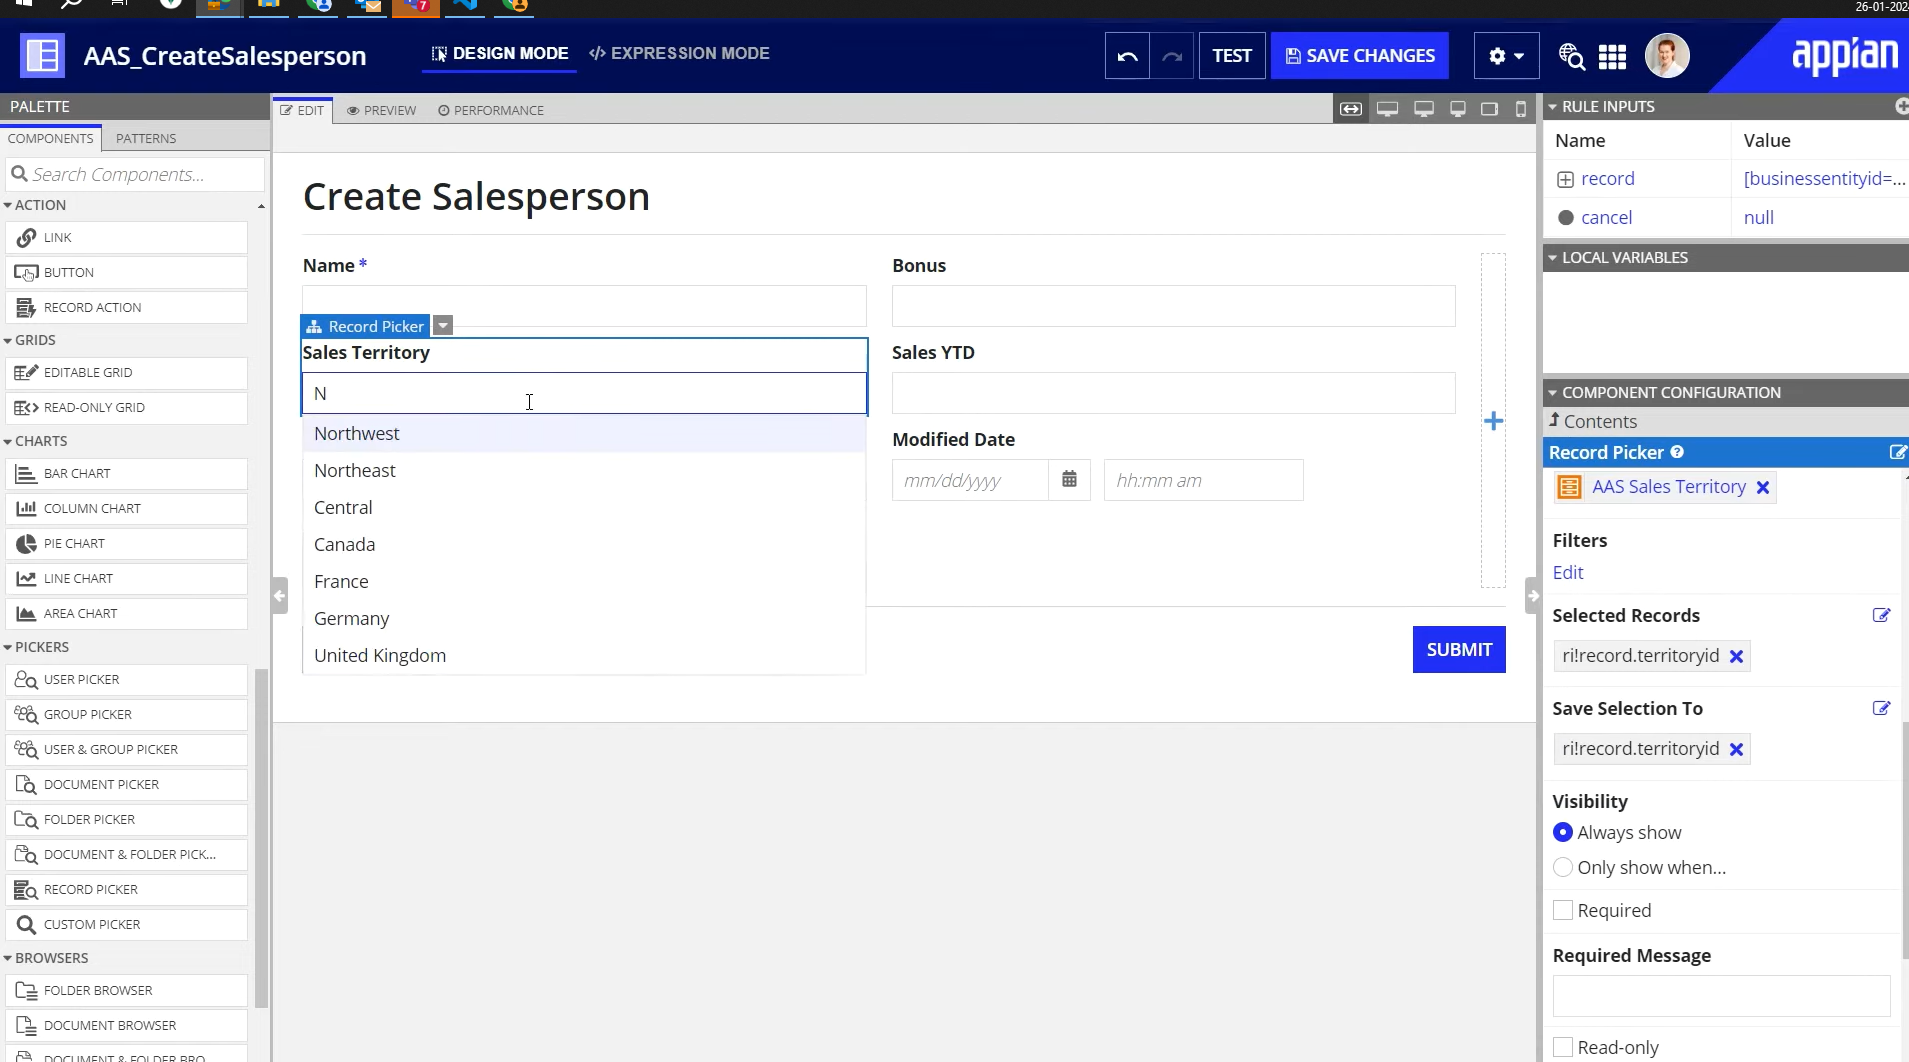
\includegraphics[width=\textwidth]{imgs/AppianUI.png}
            \caption{Appian UI}\label{fig:appian-ui}
            \source{\cite{mendix-ui}}
        \end{figure}

        Appian destaca-se no mercado de desenvolvimento de software devido a várias funcionalidades distintas. Algumas delas incluem:
        
        \begin{enumerate}
            \item \textbf{Deployment Eficiente:}
                \begin{itemize}
                    \item Permite a implantação rápida de aplicações com variadas ferramentas de implantação;
                    \item Oferece a sua própria solução para controlo de versionamento.
                \end{itemize}
            
            \item \textbf{Vários Formatos para Apresentação de Dados:}
                \begin{itemize}
                    \item Possibilita apresentar dados em vários formatos, como tabelas, gráficos em formato grade e PDF.
                \end{itemize}
            
            \item \textbf{Desenvolvimento Visual:}
                \begin{itemize}
                    \item Programadores podem moldar fluxogramas para criar diagramas de processos de forma visual, eliminando a necessidade de codificar manualmente.
                \end{itemize}
            
            \item \textbf{Pontos a Considerar (Desvantagens):}
                \begin{itemize}
                    \item Processo de documentação precisa de ser aprimorado;
                    \item Limitações na integração com outros produtos;
                    \item A ferramenta de gestão de permissões pode ser um pouco lenta;
                    \item Desenvolvimento geral de aplicações pode ser mais lento em comparação com as alternativas analisadas.
                \end{itemize}
        \end{enumerate}
        
        Appian destaca-se na eficiência da implantação de aplicações e na criação de processos através de fluxogramas visuais. A sua flexibilidade na apresentação de dados, em junção com a capacidade de desenvolver aplicações para diversos setores, fazem dela uma opção bastante versátil\cite{mendix-vs-outsystems-vs-appian}.

    \subsubsubsection{Pega Platform}\label{secsecsec:pega}
    
        % fundada https://www.pega.com/about/leadership/alan-trefler#:~:text=Inspired%2C%20he%20founded%20Pega%20in,today%20known%20as%20low%2Dcode.

        A Pega Platform, a plataforma mais antiga das analisadas, fundada em 1983, foi criada por Alan Trefler, um programador na área financeira e dos seguros, fundou Pega devido à desconexão que existia entre os métodos tecnológicos usados e os processos e objetivos empresariais. Desde então, a plataforma tem desempenhado um papel crucial no cenário de desenvolvimento de software, fornecendo soluções robustas para diversas necessidades empresariais, a sua interface está representada na Figura \ref{fig:pega-ui}.

        \begin{figure}[htbp] % htbp
            \centering
            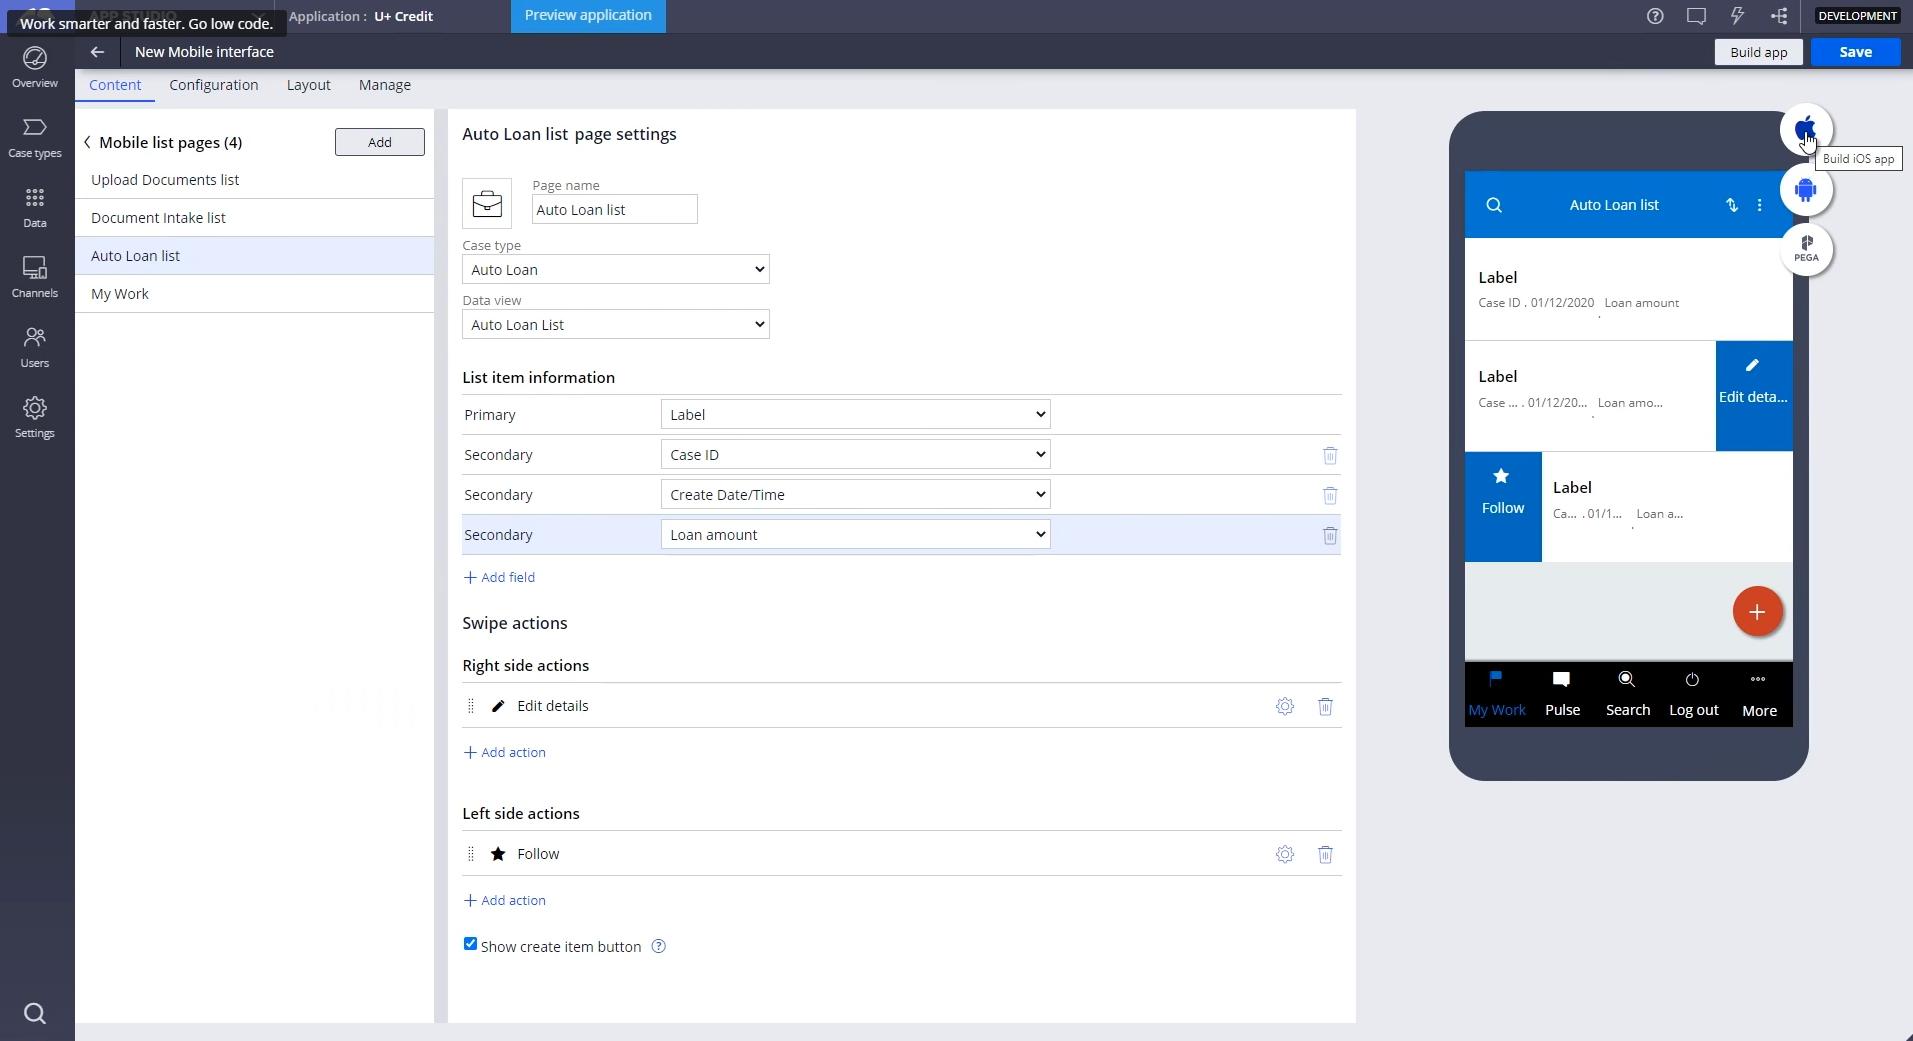
\includegraphics[width=\textwidth]{imgs/PegaUI.png} % You can replace 'example-image-a' with the path to your actual image
            \caption{Pega UI}\label{fig:pega-ui}
            \source{\cite{pega-ui}}
        \end{figure}

        Algumas vantagens e desvantagens da plataforma incluem:
    
        \begin{itemize}
        \item \textbf{Vantagens:}
            \begin{itemize}
            \item Oferece uma abordagem eficiente na gestão de casos, utilizando um modelo central que permite controlar tarefas, contribuindo para uma integração forte com os paradigmas das empresas\cite{o-que-e-gestao-de-casos-pega};
            \item Forte capacidade de incorporar e utilizar inteligência artificial nas aplicações.
            \end{itemize}
        
        \item \textbf{Desvantagens:}
            \begin{itemize}
            \item Tem uma curva de aprendizagem mais acentuada.
            \end{itemize}
        \end{itemize}    

        \subsection{ServiceNow}\label{sec:service-now}

            \begin{figure}[htbp]
                \centering
                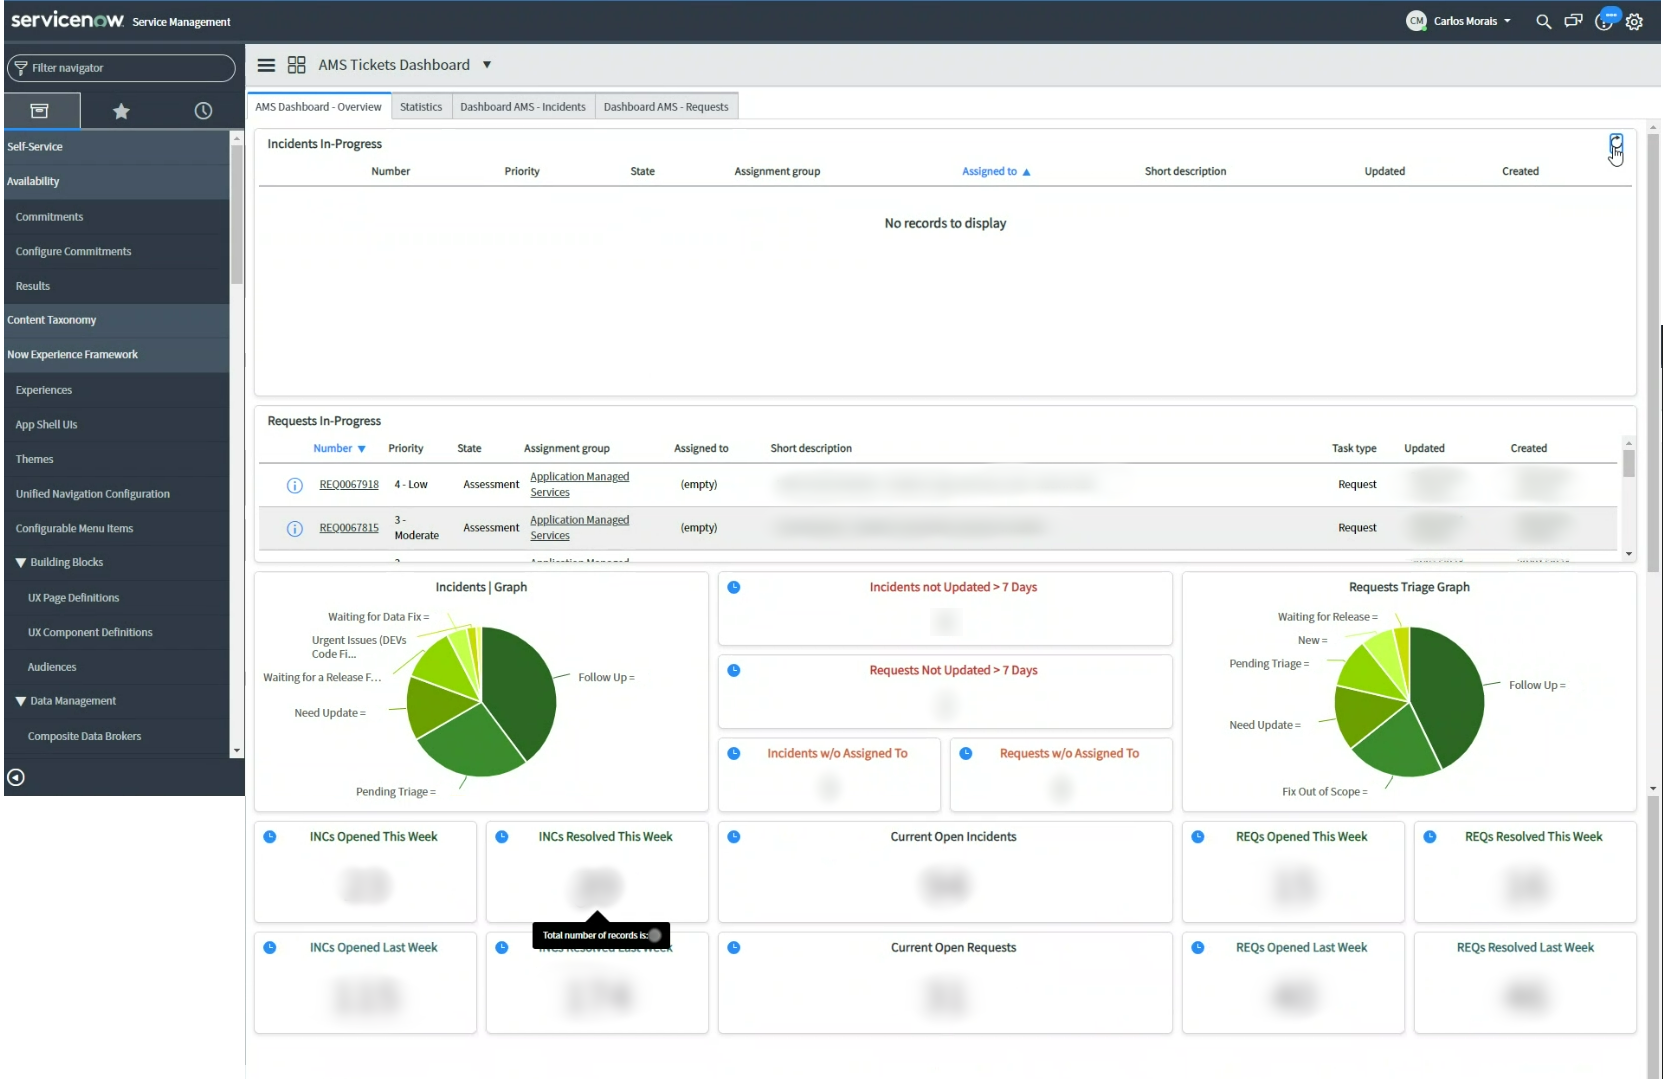
\includegraphics[width=\textwidth]{imgs/ServiceNow.png} % You can replace 'example-image-a' with the path to your actual image
                %\caption{Plataforma ServiceNow - Pagina Principal}
                \caption[Plataforma ServiceNow - Pagina Principal]{Plataforma ServiceNow - Pagina Principal\protect\footnotemark}\label{fig:service-ui}
                \source{Plataforma Interna da ServiceNow}
            \end{figure}
            \footnotetext{alguma da informação nesta e em próximas imagens será censurada devido a questões de confidencialidade.}

            A ServiceNow é uma das plataformas de referência na gestão de serviços empresariais, oferecendo uma ampla gama de funcionalidades para otimizar e automatizar processos internos. Destaca-se pela sua capacidade de integrar e gerir eficientemente serviços de TI, recursos humanos, gestão de projetos e muito mais, a página principal da aplicação está demonstrada na Figura \ref{fig:service-ui}. Fundada em 2004 pelo antigo CTO da Peregrine Systems, Fred Luddy, ServiceNow iniciou a sua existência num único computador portátil, numa pequena sala de escritório, apoiada por um único colaborador e um punhado de voluntários dedicados.

            A partir destes começos, Luddy propôs-se a criar uma plataforma baseada na nuvem para encaminhar o trabalho de forma eficaz, sendo suficientemente poderosa para impulsionar o sucesso empresarial, mas, simultaneamente, simples o suficiente para não afastar potenciais utilizadores. Não é surpreendente que este objetivo tenha chamado a atenção dos clientes. A empresa cresceu rapidamente e, em 2012, tornou-se pública.
            
            Desde então, ServiceNow expandiu significativamente as suas ofertas, e as mesmas prioridades que definiram a sua fundação há vinte anos continuam a defini-lo hoje: uma paixão por fazer as pessoas tirarem mais proveito da tecnologia. 
            
            Atualmente, as ofertas da ServiceNow incluem gestão de serviços de IT, gestão de operações de IT, gestão de serviços ao cliente, gestão de recursos humanos, operações de segurança, risco e conformidade, entrega de serviços no local de trabalho e gestão de serviços de campo - tudo numa só plataforma.

            É através da ServiceNow que os utilizadores reportam os dois tipos de incidentes, request ou incidente, como explicado na secção \ref{sec:terminologia_do_projeto}. De seguida estes passam por uma equipa de suporte que tenta filtrar e resolver os incidentes mais simples, como utilizadores a utilizar mal a plataforma, ou por vezes incidentes que a equipa de desenvolvimento os instruiu a resolver, por exemplo, se um certo problema aparecer, instruam os utilizadores a apagar a cache do browser. Após esta fase, se não foi possível resolver, são enviados para a ServiceNow onde são analisados pelo team leader da equipa em triagem, que manda uma mensagem padrão para o utilizador a pedir desculpas pela inconveniência e a informar que se está investigar o problema, e prioriza os incidentes da seguinte forma:
            \begin{itemize}
                \item \textbf{Low} - Um erro de baixa importância que não bloqueia o utilizador, como uma desformatação do site;
                \item \textbf{Medium} - Quando é mais urgente no sentido de poder afetar a funcionalidade da plataforma, mas haver como contornar o problema, como recarregar a página ou refazer o contrato;
                \item \textbf{High} - Quando o utilizador está bloqueado e não consegue aceder à funcionalidade que necessita. Esta prioridade também pode ser dada a utilizadores de certas organizações maiores, no sentido de serem clientes mais importantes que a empresa quer garantir que mantém;
                \item \textbf{Critical} - Prioridade atribuída a erros urgentes, como erros 502, qundo o site está em baixo e ninguém conseguir aceder.
            \end{itemize}
            Seguidamente, ao longo da vida de um incidente este será movido entre um dos seguintes estados, como se pode ver na Figura \ref{fig:servicenow-ui2}:
            \begin{itemize}
                \item \textbf{New:} Novo — O estado inicial de um incidente que acabou de ser recebido;
                \item \textbf{Pending Triage:} Pendente de Triagem — Aguarda avaliação;
                \item \textbf{Waiting for Data Fix:} Aguardando Correção de Dados — À espera que o \textit{datafix}, pedido à equipa da base de dados, seja efetuado;
                \item \textbf{Urgent Issues (DEVs):} Problemas Urgentes (DEVs) — Incidentes críticos que requerem atenção imediata dos programadores;
                \item \textbf{Need update:} Necessita de Atualização — Requer atualização ou informação adicional como por exemplo o UMR (Unique market reference) para identificar o contrato problemático do utilizador;
                \item \textbf{Follow up:} Acompanhamento — À espera de feedback do utilizador para saber se o problema foi resolvido;
                \item \textbf{Follow up second strike:} Acompanhamento segundo golpe — Segundo a política da empresa, após vinte e quatro horas volta-se a mandar mensagem ao utilizador e se nas vinte e quatro seguintes ainda não houver resposta, fecha-se o incidente;
                \item \textbf{Waiting for release:} Aguardando Lançamento — Foi criado \textit{defect} a partir do incidente e espera-se que seja lançada a versão com a correção para produção.
            \end{itemize}
            
            \begin{figure}[htbp]
                \centering
                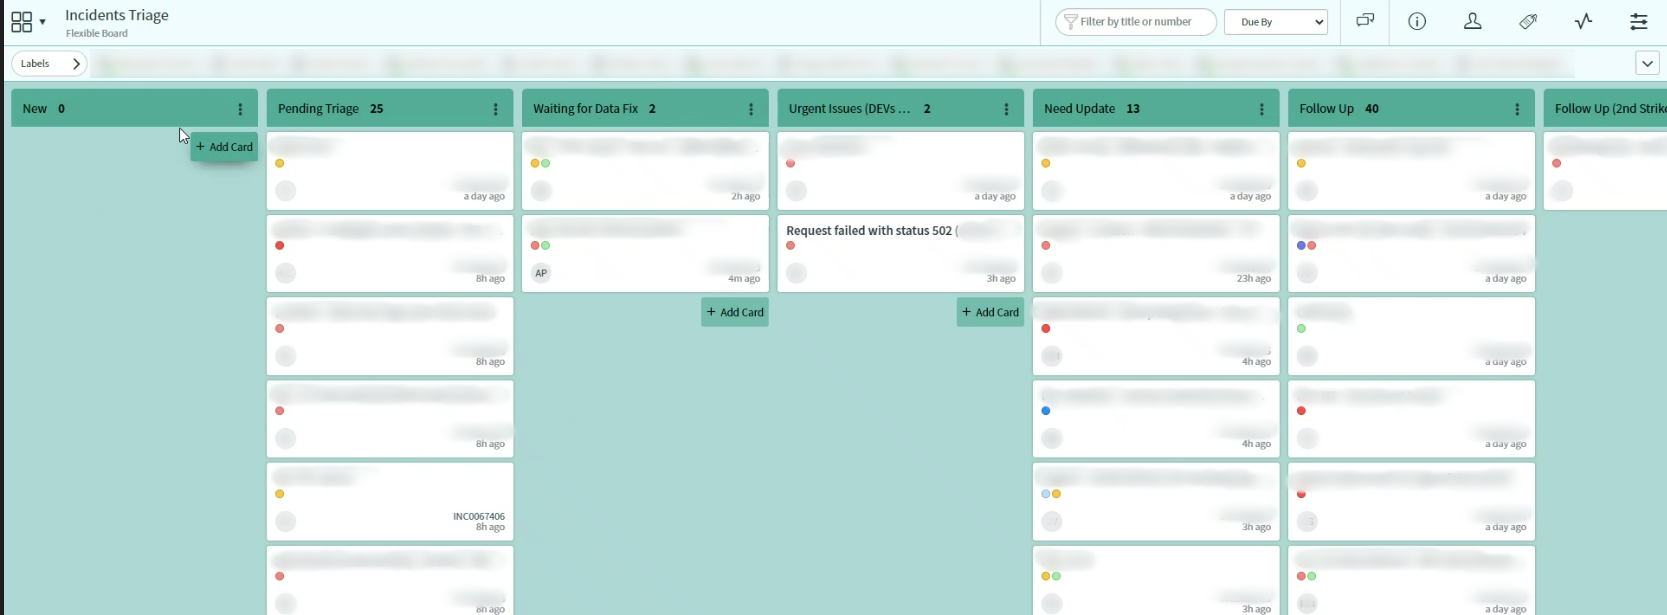
\includegraphics[width=\textwidth]{imgs/ServiceNow2.png}
                \caption{Plataforma ServiceNow - Incidentes}\label{fig:servicenow-ui2}
                \source{Plataforma Interna da ServiceNow}
            \end{figure}

            \subsubsection{Competidores}\label{competidores-service-now} % devo manter, devo arranjar alternativas mesmo? todo
        
                Neste ambiente altamente volátil e de alta competição no desenvolvimento de software empresarial existirão sempre ferramentas que podem substituir funcionalidades de outras, no entanto, no caso da ServiceNow é difícil encontrar uma que faça exatamente o que esta plataforma faz. 
                
                Na realidade o que se alcança com a plataforma ServiceNow pode ser já alcançado pelas ferramentas usadas como o Jira ou Confluence ou por outras como ClickUp[\ref{clickup}], mas a verdadeira vantagem da ServiceNow é a habilidade de ter tudo no mesmo sítio, sendo por isso uma ferramenta única na gestão empresarial.

    \subsection{Plataforma Atlas}\label{sec:ferramentas-atlas}

        \begin{figure}[htbp]
            \centering
            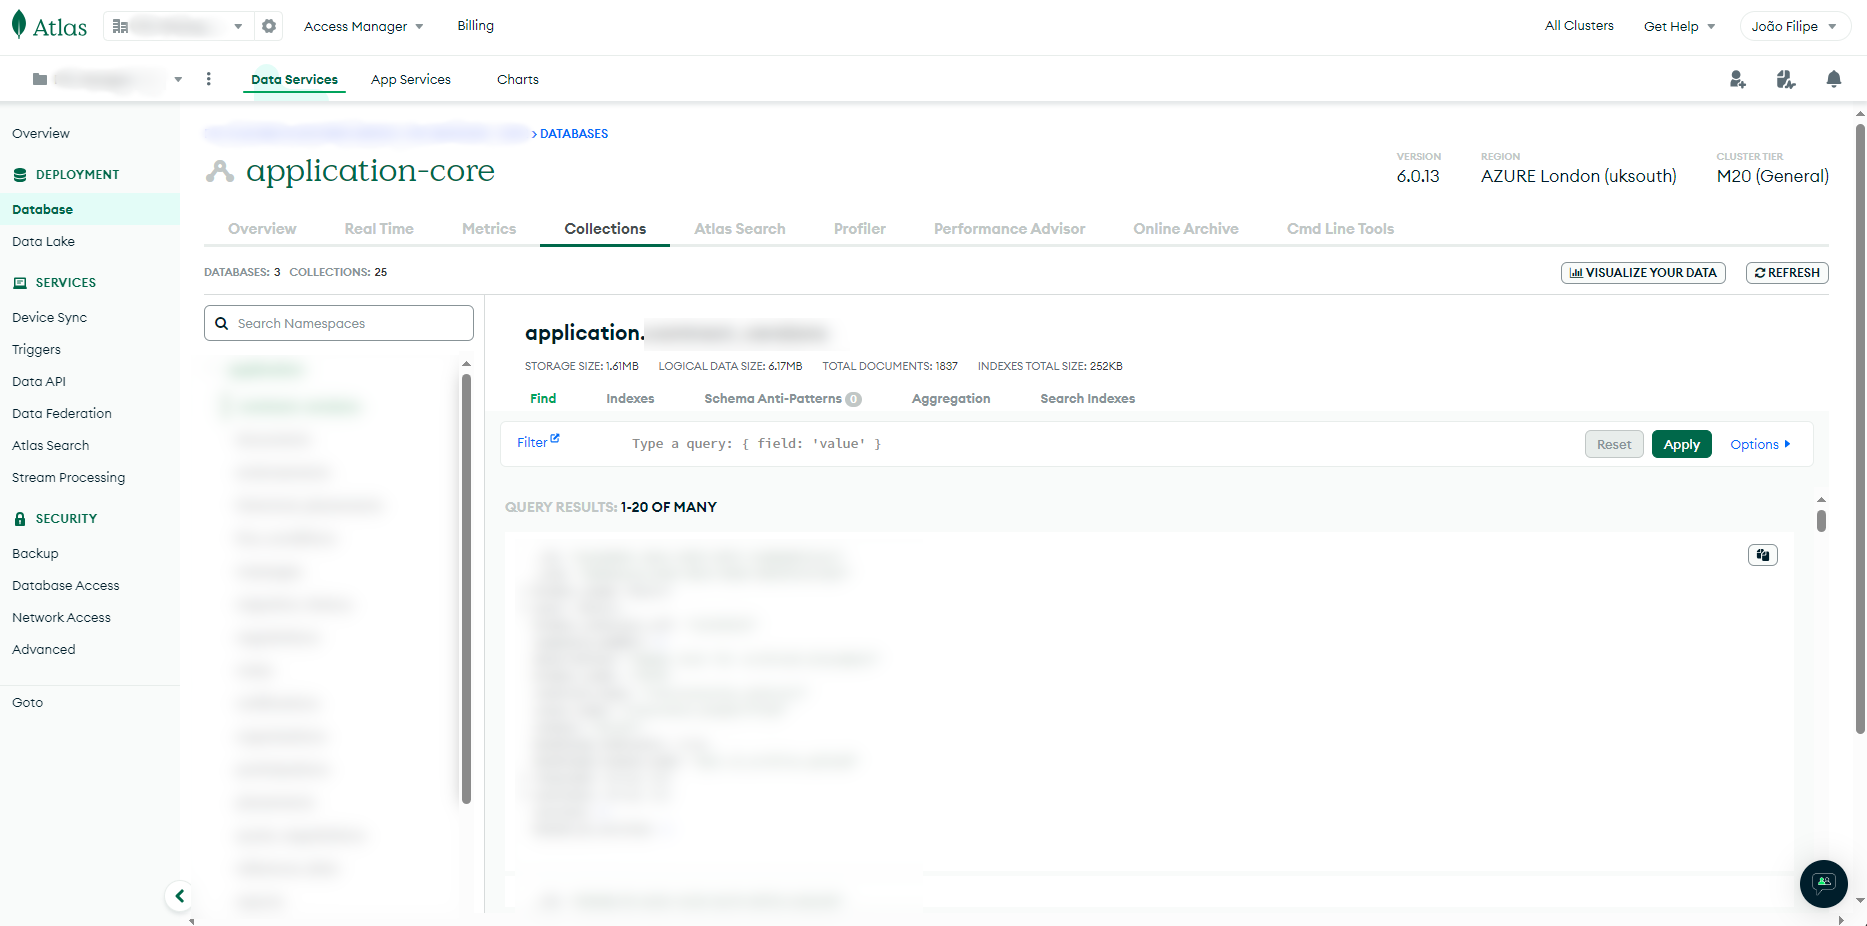
\includegraphics[width=\textwidth]{imgs/MongoDB.png} % You can replace 'example-image-a' with the path to your actual image
            \caption{Plataforma Atlas}\label{fig:atlas-ui}
            \source{Plataforma Interna do Atlas}
        \end{figure}

        Atlas, cuja interface se pode ver na Figura \ref{fig:atlas-ui}, é um componente crucial do processo, e é uma das plataformas mais usadas no que toca à resolução e análise de problemas.  
        
        A plataforma está integrada com todos os ambientes do projeto, permitindo escolher entre estes no canto superior esquerdo. Existem, no entanto, algumas restrições, por exemplo, para se poder ter acesso ao ambiente de produção, é necessário aceder primeiro à \hyperref[sec:plataforma-azure]{Plataforma Azure}, aceder a ``My roles'' > ``Groups'' e Pedir acesso com um campo para mencionar o número do Incidente em produção que vai ser analisado e uma pequena descrição.

        Um dos campos mais usados na plataforma é o dos filtros, visível na Figura \ref{fig:atlas-ui} onde é possível filtrar por campos específicos, organizar por data, colocando no campo ``sort'' por exemplo \texttt{\{``\_metadata.modified\_date'': -1\}} ou usar ``Aggregators'', na aba relacionada que permite a criação de pesquisas complexas passo a passo, removendo alguma dessa complexidade.

        É também aqui onde se gerem algumas das permissões relacionadas com a Base de Dados, ações reservadas apenas a alguns profissionais por questões de segurança. 
            
        \subsubsection{Competidores}\label{competidores-atlas}

            Em vez de uma base de dados NoSQL, a plataforma poderia beneficiar de uma base de dados SQL, até devido à melhor integração com outras ferramentas e à maturidade do mercado.

            Pelo que uma das alternativas a baixo tratadas é uma base de dados SQL.

            \subsubsubsection{Cosmos DB}\label{cosmos-db}

                Visto que é parte do ambiente Azure que já é extensivamente utilizado, seria mais fácil integrar com o projeto. Isto não quer dizer que uma transição seria fácil, normalmente transições deste tipo têm que ser muito bem justificadas devido aos preços e mão de obra exigidos.

                A escolha entre Cosmos DB e MongoDB depende das necessidades específicas da empresa. Cosmos DB destaca-se quando se necessita de flexibilidade com múltiplos modelos de dados, enquanto que o MongoDB se concentra no modelo de documentos. Cosmos DB oferece escalabilidade global e replicação automática em várias regiões, tornando-se ideal para baixa latência e elevada disponibilidade\cite{cosmosdb-vs-mongodb}.

            \subsubsubsection{MariaDB}\label{amazon-web-services}

                Esta seria uma solução que manteria um paradigma NoSql como o MongoDB. 

                MariaDB, uma base de dados relacional, adota o formato de tabela testado pelo tempo. Cada tabela no MariaDB segue um esquema fixo, definindo meticulosamente as colunas e os respetivos dados. Esta forma metódica de armazenar dados não apenas garante precisão, mas também estabelece estruturas predefinidas, fomentando clareza e organização o que contrasta com a utilização mais relaxada de BSON para armazenar dados em MongoDB.

    \subsection{Plataforma Azure}\label{sec:plataforma-azure}

        \begin{figure}[htbp]
            \centering
            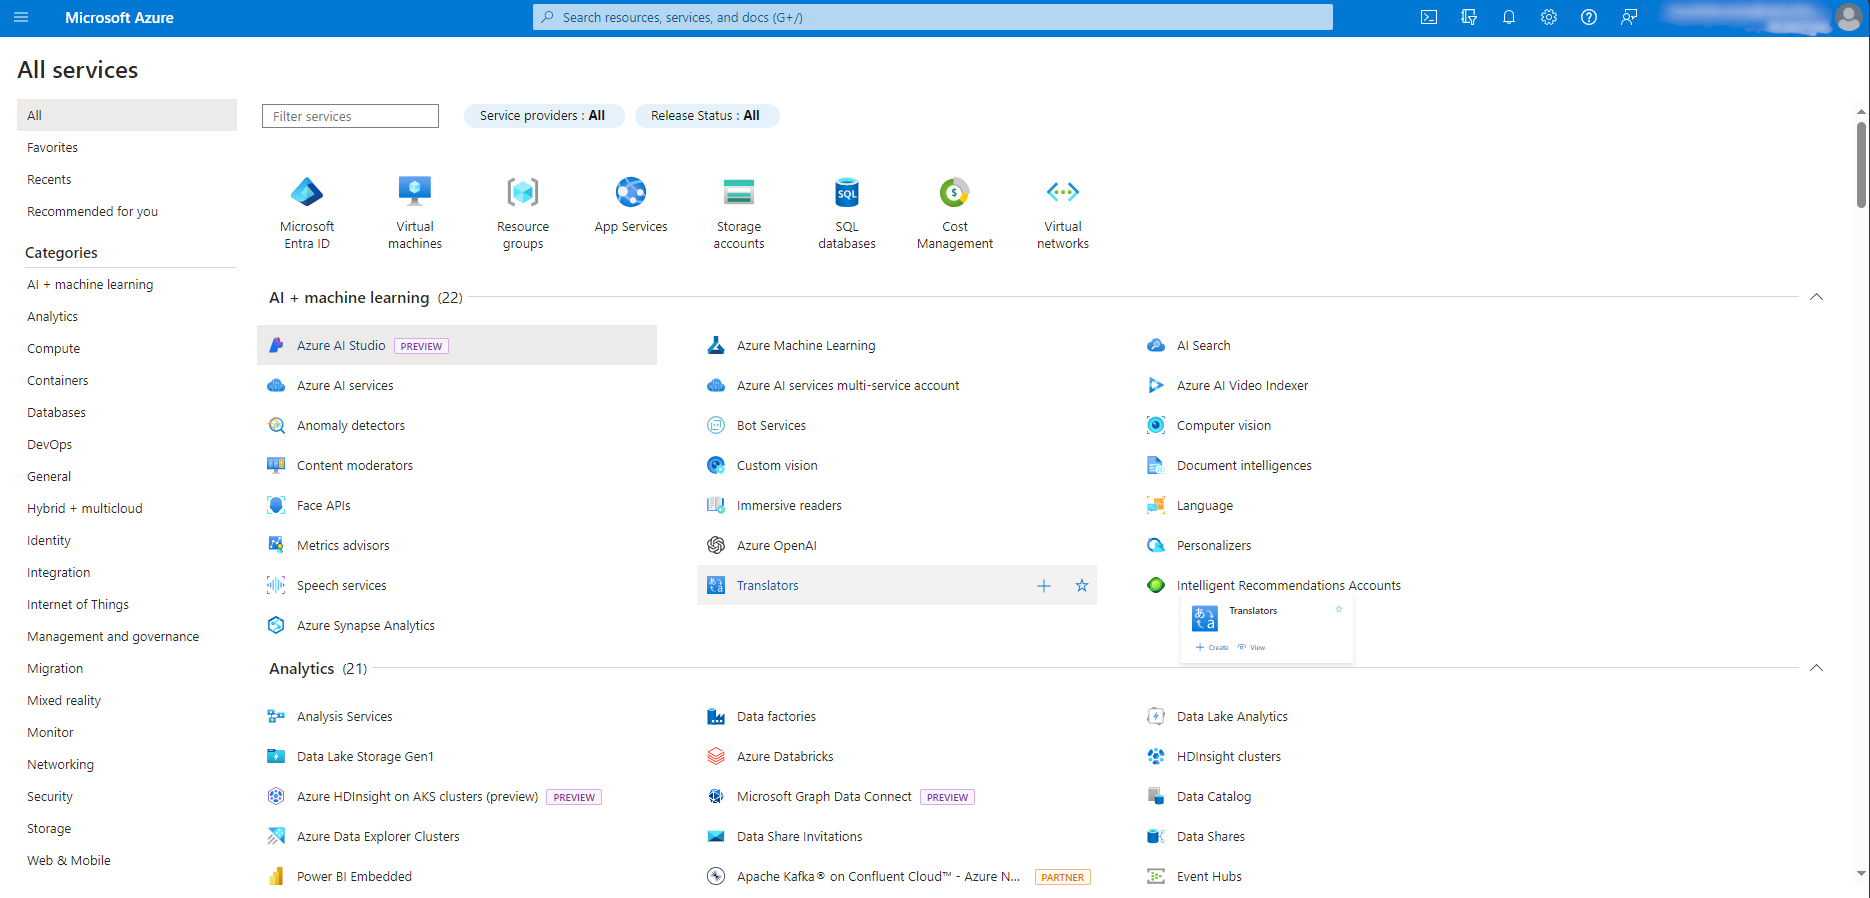
\includegraphics[width=\textwidth]{imgs/Azure.png}
            \caption{Plataforma Azure}\label{fig:azure-ui}
            \source{Plataforma Interna Azure}
        \end{figure}

        A plataforma Azure é a que engloba mais operações e áreas distintas do projeto, desde segurança até à gestão das máquinas virtuais usadas para os ambientes.

        Existe uma panóplia enorme de serviços, como é visivel na Figura \ref{fig:azure-ui}, estes incluem ``logic apps'', ``azure storage'', ``storage accounts'', ``Azure Virtual Network'' e ``Azure Health'', etc. Alguns dos que são mais usados e geridos na plataforma são os seguintes:

        \subsubsection{Resource Groups}

            Os \textit{Resource Groups} desempenham um papel crucial na organização e gestão eficiente dos recursos. Permitem agrupar recursos relacionados, como recursos relacionados com ambientes diferentes. Ao utilizar estes grupos, a administração torna-se também mais fácil e permite políticas de segurança e controle de acessos a grupos específicos. 

        \subsubsection{Virtual Machines}

            É na gestão de Máquinas Virtuais do Azure que é possível aplicar os conceitos de \textit{scale out} e \textit{scale up} discutidos na Secção \ref{secsec:azure}, muitas vezes necessário para fazer um deployment específico ou devido a fluxos invulgares de utilizadores para a plataforma. É nesta secção que se monitoriza o seu desempenho, se aplicam atualizações e se configuram as definições necessárias.

        \subsubsection{SQL Database} % perguntar ao Marcio o 

            A secção de SQL Database no Azure é essencial para a gestão e análise, manual ou automática, de bases de dados e outros problemas gerados pelas diferentes plataformas. É aqui que se tem acesso a todas as ferramentas avançadas do Azure para analisar os dados que podem ter vindo de qualquer ponto da plataforma.

        \subsubsection{Competidores}\label{competidores-azure}

            Devido à magnitude de serviços e funcionalidades que o Azure providencia, é difícil encontrar uma alternativa que disponha de todas as mesmas ferramentas, ou não tenha as suas próprias funcionalidades diferentes. Mas algumas ferramentas que podem ser consideradas são as seguintes:

            \subsubsubsection{Amazon Web Services(AWS)}\label{competidores-aws}

                O Amazon Web Services (AWS) é uma plataforma de nuvem também bastante usada no mercado, visto que a sua empresa mãe é a Amazon. Oferece uma ampla gama de serviços e soluções para atender às necessidades de organizações de todas as dimensões. Lançada em 2006, a AWS tornou-se rapidamente numa referência para o setor.

                A escolha entre Azure e AWS é depende muito das necessidades da empresa, por exemplo, uma empresa que precise de melhor integração com o Windows ou com PaaS, poderá estar melhor com o Azure, enquanto uma que necessite mais de IaaS, poderá estar melhor com a AWS.
                
                Ambas as ferramentas oferecem basicamente as mesmas funcionalidades, mas a AWS mantém-se a líder a termos de adoção global a 33\% enquanto o Azure se mantém apenas com 13\%\cite{aws-vs-azure}.

            \subsubsubsection{Oracle Cloud}\label{competidores-oraclecloud}

                A Oracle Cloud é também uma plataforma de nuvem proeminente no mercado, pertencente à Oracle Corporation e lançada em 2016\cite{launch-orcale-cloud}, incluindo serviços de computação, armazenamento, bases de dados (podendo servir também como alternativa ao Atlas), inteligência artificial, blockchain, etc. Também com um foco especial em aplicações empresariais.

                Tem um plano grátis que permite até acesso ilimitado a uma pequena máquina virtual, atraindo de inicio muitos pequenos negócios e empreendedores individuais.

                É também uma plataforma com serviços IaaS mais em foco, e mantém uma adoção de cerca de 8.43\%\cite{marketshare-oracle-cloud}.

    \subsection{Plataforma MS Teams}
    
        \begin{figure}[htbp]
            \centering
            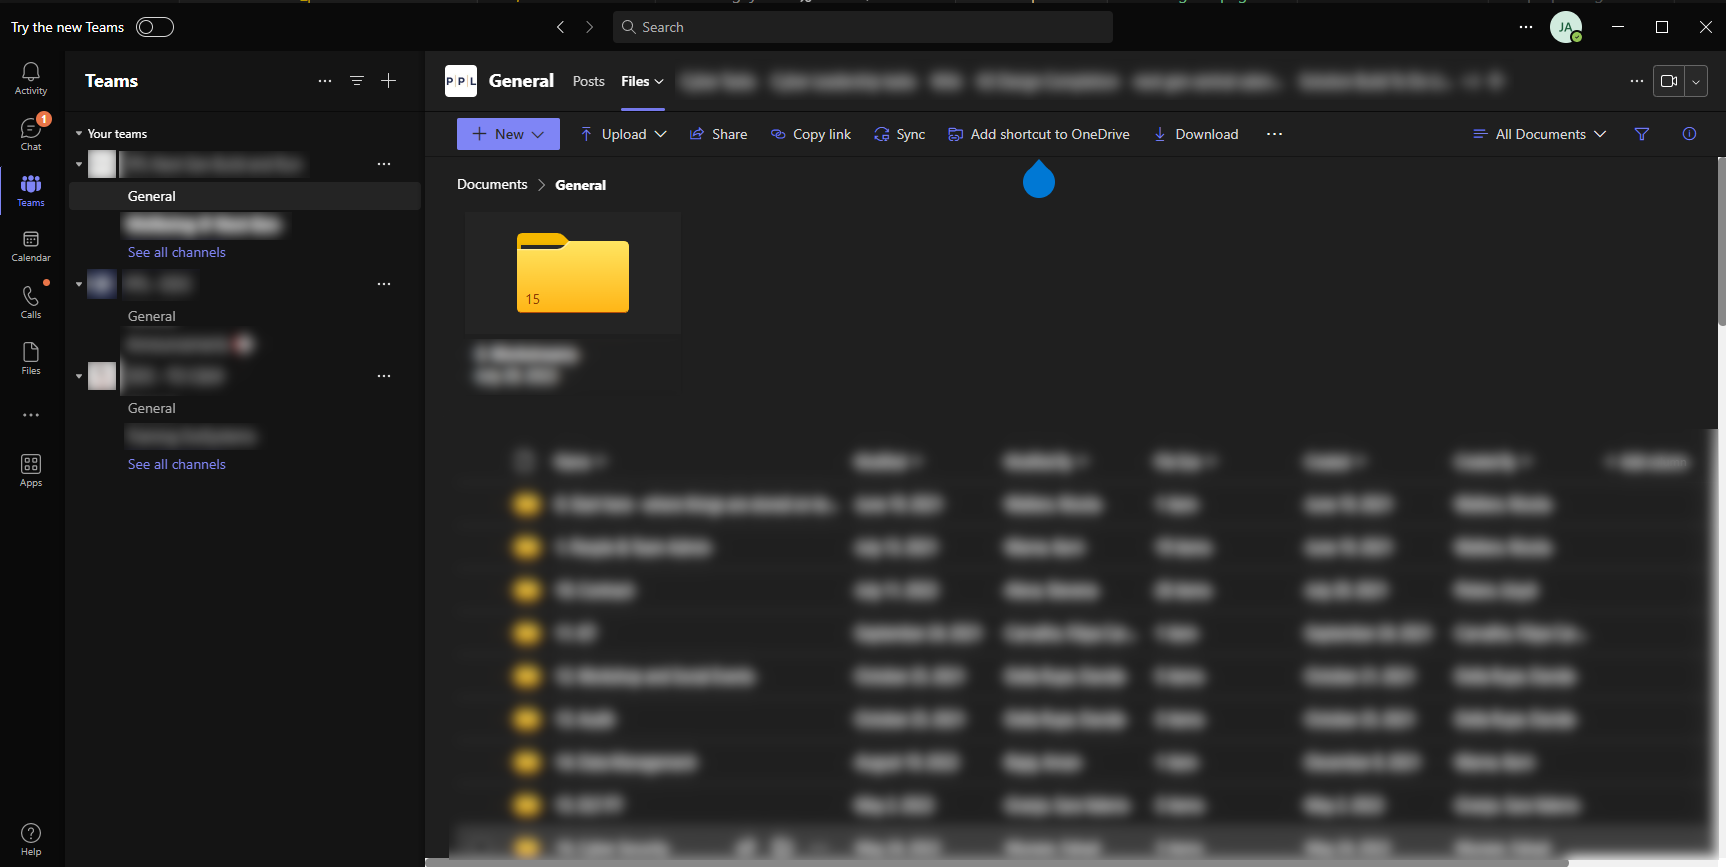
\includegraphics[width=\textwidth]{imgs/MSTeams.png} % You can replace 'example-image-a' with the path to your actual image
            \caption{Plataforma do Microsoft Teams}\label{fig:msteams-ui}
            \source{Plataforma Interna do Microsoft Teams}
        \end{figure}

        O Microsoft Teams é uma ferramenta essencial para a colaboração e comunicação eficaz na equipa. É onde acontece a maior parte da comunicação em tempo real por mensagens instantâneas, chamadas de áudio e vídeo, e colaboração em documentos em tempo real, tornando a componente geográfica transparente. É também onde se partilham muitos documentos e vídeos importantes para a organização do projeto, desde documentos Excel, como as férias de cada contratado, como vídeos gravados de formação dos KTs. Na Figura \ref{fig:msteams-ui} pode-se ver a página principal com as váreas equipas de que um traballhador faz parte à esquerda.
        %  (falados na secção \ref{sec:estrutura-organizacional-da-ril-na-deloitte-PT})
            
        \subsubsection{Competidores}\label{competidores-msteams}

        Visto que o MS Teams está intimamente integrado com muitas das ferramentas usadas diariamente, como o cliente de e-mail, Outlook, ou o calendário, ou SharePoint para partilha de ficheiros, é preciso considerar alternativas que ofereçam também estas ferramentas, ou permitam uma integração fácil com as mesmas.

            \subsubsubsection{Slack}\label{competidores-slack}

                O \href{https://slack.com/}{Slack} é uma plataforma de comunicação empresarial, permite a criação de canais para discussões específicas, integração com diversas ferramentas como calendários, permitindo que eventos sejam visualizados diretamente na plataforma. É possível partilhar documentos e ficheiros diretamente, mas não existe uma aba ou sítio onde se possam colocar ficheiros para todos os membros verem, para isto seria necessária uma solução de armazenamento externo como Google Drive ou SharePoint.
                
                Quanto aos preços, o Slack oferece uma versão gratuita com funcionalidades básicas e um histórico de mensagens limitado. As opções pagas, como o Slack Plus e o Slack Enterprise Grid, proporcionam funcionalidades avançadas, armazenamento adicional e suporte.

            \subsubsubsection{NextCloud Stack}\label{competidores-nextcloud}

                O \href{https://nextcloud.com/}{NextCloud} é a melhor alternativa no mercado de código aberto, oferece serviços como calendário, vídeo-chamadas, mensagens, listas \textit{to-do}, partilha de ficheiros, colaboração em ficheiros em tempo real, tudo isto em código aberto e livre de ser vetado, sendo uma boa alternativa para quem queira correr os próprios servidores, havendo também, no entanto, a possibilidade de pagar à empresa para usar os seus serviços na nuvem para correr a plataforma.

                Devido à natureza aberta da plataforma, existe uma comunidade vibrante que a rodeia, pelo que existem muitas extensões abertas feitas pela comunidade, havendo uma solução para quase qualquer funcionalidade que possa requerer, mas sendo estas funcionalidades desenvolvidas por indivíduos e não necessariamente equipas com um processo bem definido de desenvolvimento, podem muitas vezes não ser tão robustas como as funcionalidades base da plataforma.

    \subsection{Jira \& Confluence}\label{fuck_confluence_jira}

        Jira e Confluence são as ferramentas padrão da indústria para gestão de projetos ágeis e documentação colaborativa, respetivamente. A sua popularidade advém não apenas da sua robustez e fiabilidade, mas também da forma como se complementam, em parte por serem ambas desenvolvidas pela mesma companhia, Atlassian, oferecendo uma abordagem holística para o desenvolvimento de software e colaboração em equipa.

        Atlassian foi inicialmente fundada em 2002 por Mike Cannon-Brookes e Scott Farquhar como uma empresa que oferecia suporte a outras empresas, mas o software para gestão dos incidentes e defeitos usado na altura não era muito promissor, pelo que desenvolveram a sua própria ferramenta: JIRA. Criaram também um modelo de negócio para o desenvolvimento e venda desta ferramenta e, mais tarde em 2004, desenvolveram também o Confluence\cite{20-years-atlassian}.

        % Parágrafo sobre a Integração entre Jira e Confluence
        A integração entre Jira e Confluence forma uma poderosa sinergia, esta integração é notável em algumas funcionalidades como: ser possível adicionar incidentes da Jira diretamente na documentação do Confluence que são atualizados automaticamente, criar uma página do Confluence diretamente a partir das páginas da Jira, adicionar o estado de projetos da Jira no Confluence através de dashboards ou templates, ou adicionar novos incidentes diretamente através do Confluence ao sublinhar texto. 

        \subsubsection{Plataforma Jira}\label{secsec:jira}

            \begin{figure}[htbp]
                \centering
                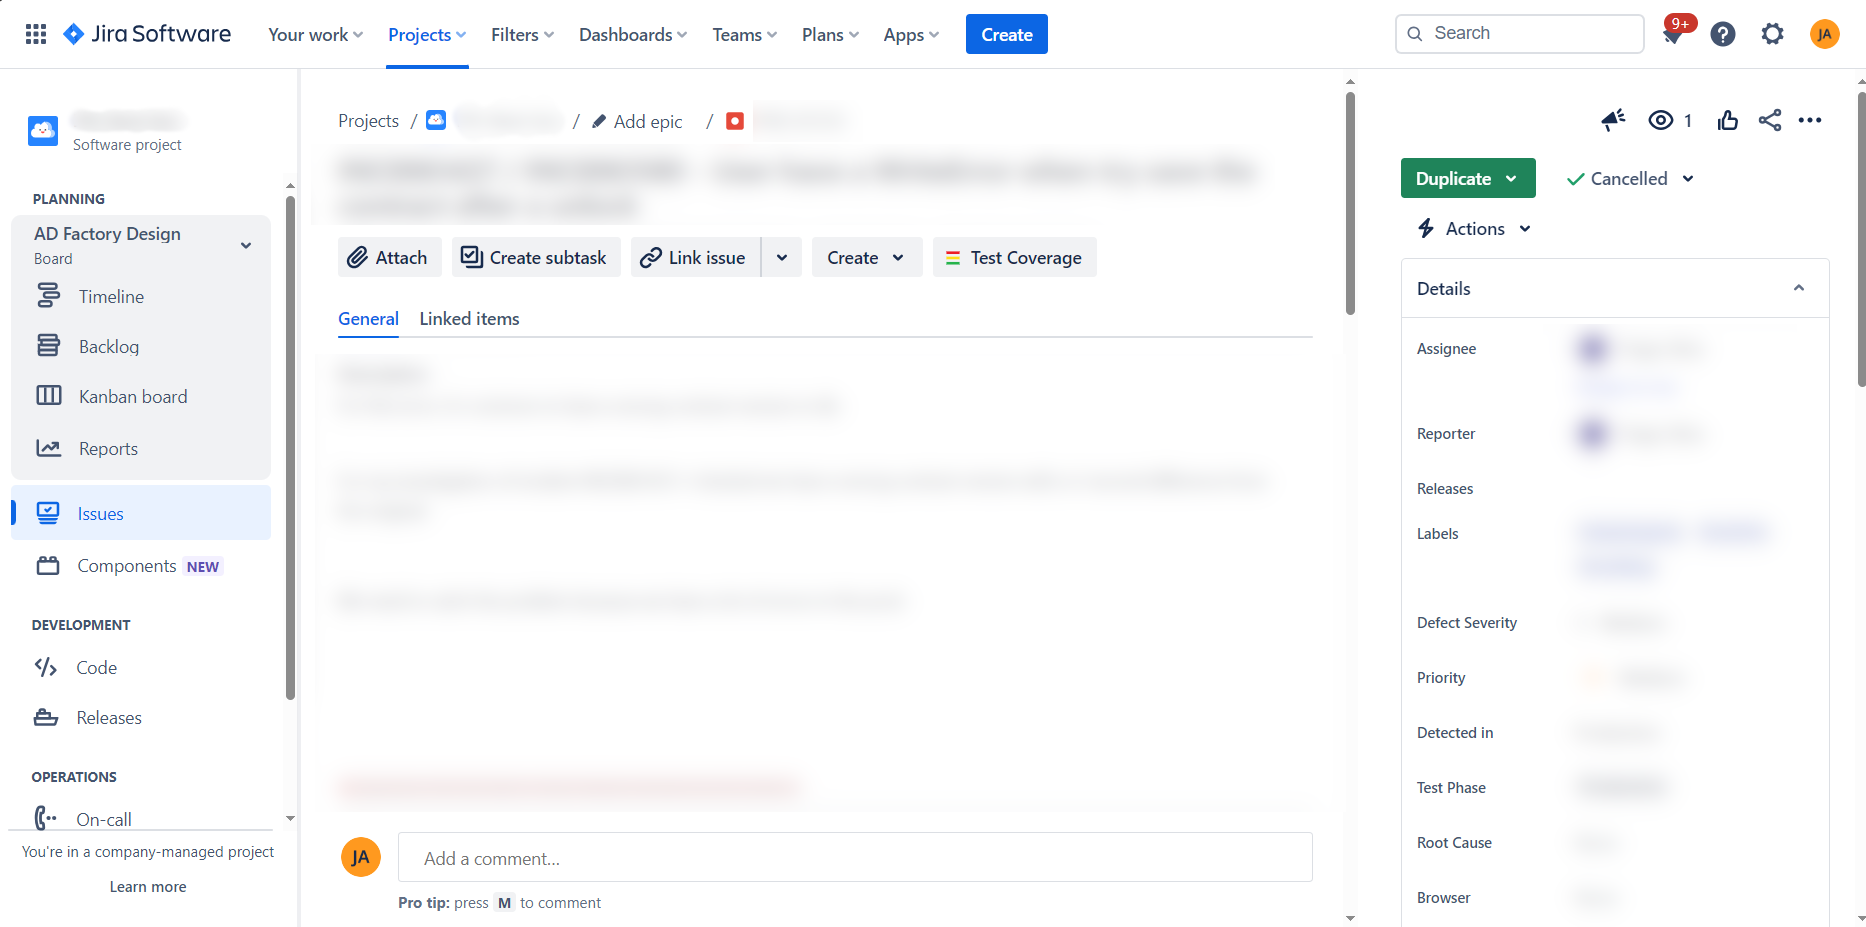
\includegraphics[width=\textwidth]{imgs/JiraSoftware.png} 
                \caption{Plataforma Jira Software}\label{fig:jira-ui}
                \source{Plataforma Interna da Jira}
            \end{figure}

            % Parágrafo sobre Jira
            A Jira facilita o desenvolvimento em metodologias ágeis, e é muito usada no projeto para manter um registo dos \textit{defects} existentes e em que estado se encontram, cada um identificado por um ID específico \textit{PNG-<XXXX>}, juntamente com o ID do incidente de que provieram se tiver sido esse o caso: \textit{INC-XXXXXX}. Existe um fluxo de estados, mostrado na Figura \ref{fig:defect-workflow}, pelo qual cada \textit{defect} tem que passar, começando no estado \textit{New} e acabando em \textit{Closed}, \textit{Duplicate} ou \textit{Rejected}. Na Figura \ref{fig:jira-ui} é possível ver interface da plataforma para a visualização de um \textit{defect}.

            \begin{figure}[htbp]
                \centering
                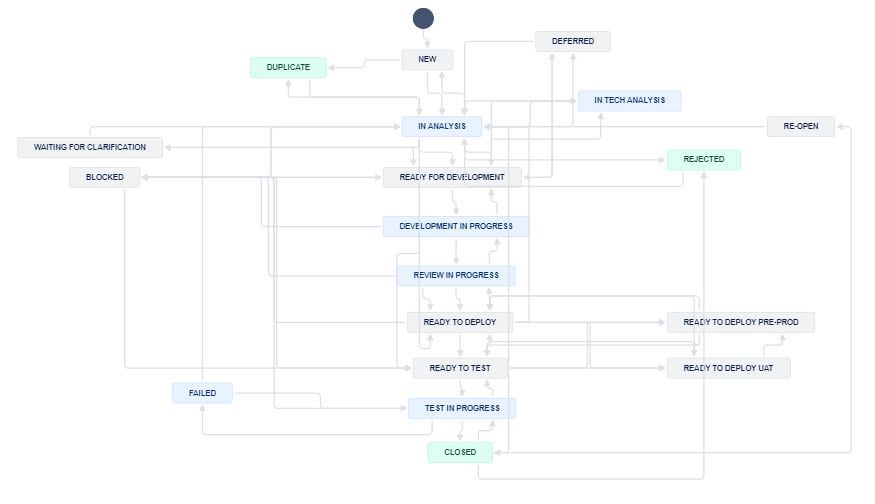
\includegraphics[width=\textwidth]{imgs/NextGenDefectWorkflow.png}
                \caption{RIL Next Gen \textit{Defect} workflow}\label{fig:defect-workflow}
                \source{Plataforma da Jira Interna}
            \end{figure}

            Em cada \textit{defect} pode-se também adicionar uma lista de \textit{subtasks} necessário completar, muitas vezes designados a diferentes membros da equipa ou até de equipas diferentes, por exemplo: \textit{Merge} do código para um ambiente específico, revisão do código, ou cenários de teste a executar. Cada \textit{subtask} tem também o seu próprio fluxo, como mostrado na Figura \ref{fig:ril-nextgen-subtasks-workflow}, começando em \textit{New} e podendo acabar em \textit{Complete} ou \textit{Cancelled}.

            \begin{figure}[htbp]
                \centering
                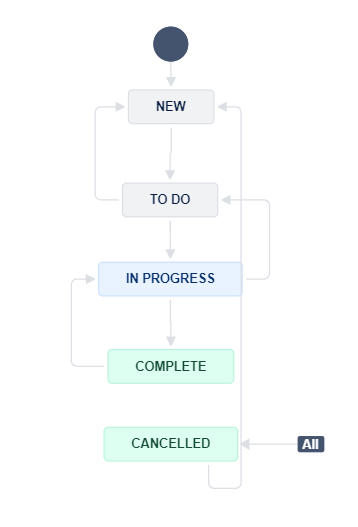
\includegraphics[scale=1.6]{imgs/NextGenSubTaskWorkflow.png}
                \caption{RIL Next Gen SubTasks workflow}\label{fig:ril-nextgen-subtasks-workflow}
                \source{Plataforma da Jira Interna}
            \end{figure}

            É possível também associar outros \textit{defects} na secção \textit{Linked Issues}, e qualquer colaborador pode deixar comentários e mencionar outros colaboradores, que irão subsequentemente receber um e-mail de aviso, permitindo fomentar um ambiente de forte e rápida comunicação.

        \subsubsection{Plataforma Confluence}\label{secsec:confluence}

            O Conflupronto, msa é isso, vou descansar um pouco, força ence é uma plataforma colaborativa de documentação e é onde a maior parte das descrições dos processos e complexidades está documentada, a sua interface é observável na Figura \ref{fig:confluence-ui}. Gere tudo desde os utilizadores de teste que se podem utilizar nos diferentes ambientes e as suas credenciais, a incidentes ou \textit{defects} que ocorrem frequentemente bem como as suas resoluções, até à documentação de como realizar certas tarefas na aplicação ou numa das plataformas de desenvolvimento.
            
            \begin{figure}[htbp]
                \centering
                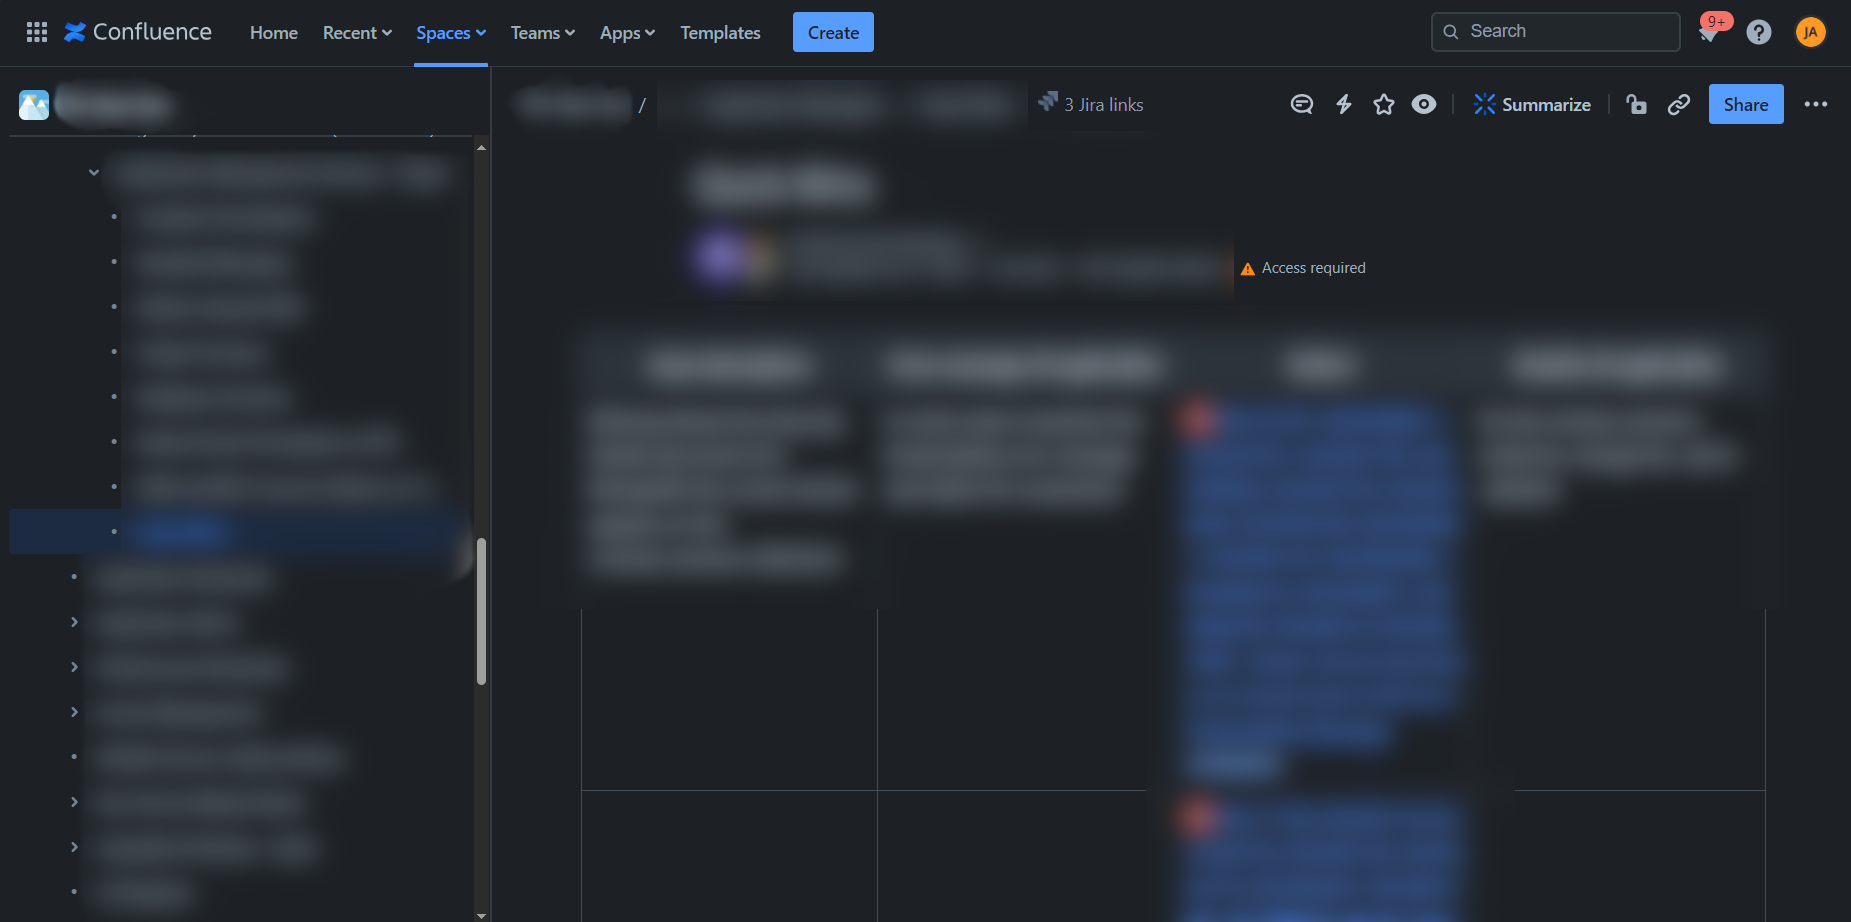
\includegraphics[width=\textwidth]{imgs/Confluence.png}
                \caption{Plataforma do Confluence}\label{fig:confluence-ui}
                \source{Plataforma do Confluence Interna}
            \end{figure}

            % Falar da agile board?
        
        \subsubsection{Competidores}\label{competidores-jira-confluence}

            Apesar de a Jira e do Confluence serem muitas vezes as ferramentas mais indicadas para a gestão de projetos, o preço destas pode ser um fator que leve a considerar outras ferramentas semelhantes, pelo que nesta secção vamos explorar algumas alternativas que possam substituir a junção do Confluence e da Jira.

        % https://www.reddit.com/r/devops/comments/10ksowi/alternative_to_atlassian_jira_and_confluence/

            \subsubsubsection{Linear + Notion}\label{linear-notion}

                \href{https://www.notion.so/}{Notion} é uma plataforma de colaboração e documentação com uma abordagem flexível e bastante personalizável mantendo uma interface simples e fácil de utilizar, permite a criação de páginas interativas, listas de tarefas, tabelas, integração com outras ferramentas como calendários e neste caso, \href{https://linear.app/}{Linear}. Esta última é uma ferramenta para desenvolvimento de software com foco no desempenho e precisão dos processos com funcionalidades como \textit{issue tracking}, listas e \textit{boards} e \textit{cycles}, uma funcionalidade que permite saber sempre qual é a tarefa em que se deve focar de seguida.
                
            \subsubsubsection{ClickUp}\label{clickup}
            
                \href{https://clickup.com/}{Clickup} é uma solução que engloba documentação e gestão de incidentes simultaneamente, é uma ferramenta que não teve tanto tempo ainda para se solidificar no mercado, mesmo em termos de integrações com outras ferramentas, mas é uma opção viável para equipas mais pequenas que procurem uma ferramenta mais simples e com um preço de entrada menor\cite{clickup-vs-jira}.

            \subsubsubsection{Bookstack + OpenProject}\label{bookstack}
            
                A alternativa de código aberto para equipas que querem garantir que o código que correm é seguro ou ter a possibilidade de contribuir diretamente ao projeto no caso de faltar alguma funcionalidade importante. Não existe, no entanto, nenhuma integração direta entre ambas as ferramentas.
                
                O \href{https://www.bookstackapp.com/}{Bookstack} é uma ferramenta de gestão de documentação que se destaca pela sua simplicidade e facilidade de uso. Oferece uma abordagem estruturada para a criação e organização de documentos.

                Já o \href{https://www.openproject.org/}{OpenProject} é uma plataforma de gestão de projetos de código aberto que oferece uma abordagem abrangente para planear, colaborar e acompanhar o progresso de projetos, permitindo uma gestão eficiente e transparente de tarefas, incidentes e equipas.